\section{Sensores}
Para navegar de manera robusta a través de entornos desconocidos y no estructurados, los robots deben poder percibir y modelar su entorno. Es por esto que lo que se busca es construir mapas precisos y ubicarse en los mismos utilizando solo sensores a bordo. A continuación se presentan algunos de los principales sensores para lograr lo propuesto.

\subsection{LiDAR}
Light Detection And Ranging, conocido como LiDAR, es una tecnología que tiene su origen en la fusión de la tecnología láser junto con la tecnología RADAR (Radio Detection And Ranging), lo cual ha permitido mejorar en gran medida la precisión de los sistemas de detección, dando lugar a nuevas aplicaciones. 

El  fundamento de los dispositivos basados en la tecnología LIDAR es el cálculo del tiempo de vuelo (\textit{ToF - Time  Of Flight}) de los pulsos láser, de manera que, conociendo la velocidad del mismo, las características angulares con las que fue emitido, y la diferencia de tiempos entre el rayo emitido y el reflejado, se puede determinar de manera sencilla la distancia a la que se encuentra el obstáculo/objeto con el que el rayo impactó. Esto permite, con gran exactitud, conocer las coordenadas de la posición de objetos o superficies con respecto del sistema de coordenadas del propio dispositivo.

Muchos investigadores tienen sensores LiDAR de exploración servo-montados en configuraciones de cabeceo [116, 117] o de barrido [118] (Fig. \ref{fig:lidars}.a) para producir exploraciones tanto planares como 3D, aunque para este último caso el mismo entrega escaneos cada 1Hz o menos. Este campo de visión, sobre todo el 3D, tiene el costo de una mayor complejidad (sincronización servo temporal) y una menor cobertura en direcciones críticas.

\begin{large}
[pfingsthron2012][newman2006][bosse2009]
\end{large}

Con el fin de aumentar la frecuencia de recolección de datos, existen sensores que integran múltiples LiDAR en una sola unidad de escaneo (Fig. \ref{fig:lidars}.b), de modo que se pueden obtener escaneados en 3D completos a altas velocidades.

\begin{figure}
    \centering
    \subfloat[Scanse Sweep]{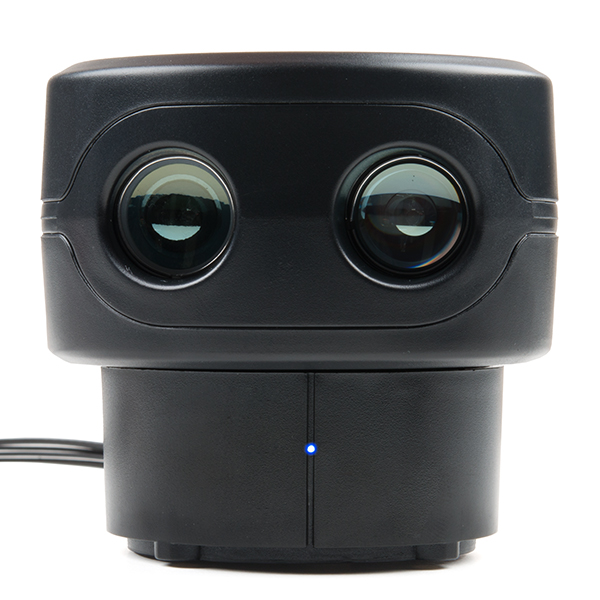
\includegraphics[width=.35\textwidth]{Img/scanse-sweep}}
    \qquad
    \subfloat[Velodyne VLP-16]{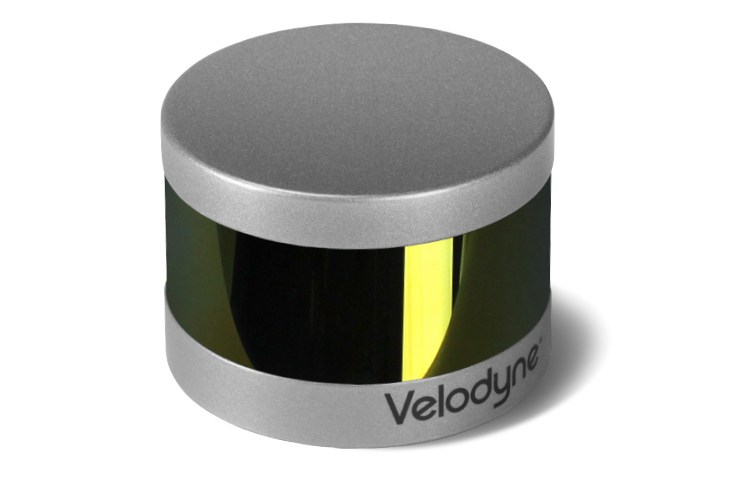
\includegraphics[width=.5\textwidth]{Img/vlp-16}}
    \caption{Algunos LIDAR comerciales}
    \label{fig:lidars}
\end{figure}

\subsection{Cámara}
Las cámaras en su versión más simple tienen la característica de ser más económicas y sencillas de montar respecto al resto de los sensores utilizados para el SLAM (tal como el LiDAR), además de no emitir señales al entorno para obtener las características del mismo. A la hora de realizar el SLAM. el modelo de sensado de las cámaras consiste básicamente en un mapeo entre el entorno tridimencional y el plano de la imagen bidimensional. Dependiendo del tipo de cámara (monocular, estéreo, omnidireccional, RGB-D, entre otras), es posible utilizar diferentes modelos matemáticos que permitan relacionar puntos del mundo con su respectiva representación en la imagen.

Para las cámaras monoculares, la línea de base entre las imágenes debe estimarse a partir de la odometría, lo que da lugar al problema de SLAM monocular bien estudiado [124, 125]. Otra forma de realizarlo es mediante la percepción de alto nivel, donde se pueden utilizar señales como el tamaño relativo de un objeto para estimar la escala de la imagen y, por lo tanto, la profundidad [126].

En cambio, para las cámaras RGB-D (\textit{D: Depth} - Profundidad) (Fig. \ref{fig:camaras}.b), uno de los métodos presentados en la literatura para la realización del SLAM a partir de las mismas [ENDERS2012] consiste en primero extraer características visuales de las imágenes de color entrantes. Luego, se comparan estas características con las características de imágenes anteriores. Al evaluar las imágenes de profundidad en las ubicaciones de estos puntos de características, se obtienen un conjunto de correspondencias 3D puntuales entre dos cuadros cualquiera. Basándose en estas correspondencias, se estima la transformación relativa entre los marcos utilizando RANSAC [TRIVEDI2013].

Por otro lado, las técnicas de visión estéreo utilizan dos cámaras con una separación entre las mismas fija y conocida (Fig. \ref{fig:camaras}.a). Las correspondencias de características de la imagen se identifican entre las imágenes mediante la geometría epipolar[REF DE CASTRO] [111], y los rangos se calculan cuando se han medido las disparidades de imagen. Los enfoques pasivos sufren desde muchos modos de falla, desde agujeros de profundidad en áreas de imagen sin características visuales, hasta escenas que crean ambigüedades [123].


\subsection{Sensores Inerciales}
El término sensor inercial se usa para denotar la combinación de un acelerómetro de tres ejes y un giroscopio de tres ejes. Los dispositivos que contienen estos sensores se denominan comúnmente unidades de medición inercial (IMU), los cuales en muchos casos incluyen tambien un magnetómetro de tres ejes. Estas unidades sensoriales suelen ser usadas para determinar la orientación y posición de objetos a los cuales se encuentran integrados, permitiendo así la incorporación de los mismos en gran número de aplicaciones [7, 59, 109, 156] [DE KOK2017].

Un giroscopio mide la velocidad angular del sensor, es decir, la velocidad de cambio de la orientación del sensor. En cambio, un acelerómetro mide la fuerza específica externa que actúa sobre el sensor. La fuerza específica consiste tanto en la aceleración del sensor como en la gravedad de la tierra. Estos sensores tienen el inconveniente de presentar un \textit{bias} variable en el tiempo que afecta su funcionamiento. Por otro lado, los magnetómetros son los encargados de medir el campo magnético en el que el objeto se encuentra sumergido, obteniendo así información absoluta del ambiente y no referida únicamente al objeto en si.

Hoy en día, muchos de estos sensores se basan en la tecnología de sistemas microelectromecánicos (MEMS). Los componentes de MEMS son pequeños, ligeros, económicos, tienen un bajo consumo de energía y tiempos de arranque cortos. Su precisión ha aumentado significativamente con los años.

\begin{figure}
    \centering
    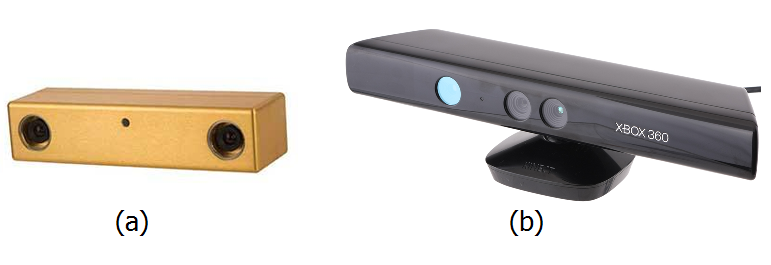
\includegraphics[width=.9\textwidth]{Img/bumblekinect}
    \caption{Cámaras: (a) Bumblebee 2, (b) Kinect}
    \label{fig:camaras}
\end{figure}

\subsection{Encoders}
El objetivo de los encoders es medir las rotaciones relativas de la rueda a la que están asociados. Los encoders normalmente se fijan a la salida del motor o de la caja de cambios, con opciones de diseño que a menudo cambian la resolución angular con la máxima velocidad. Los efectos de resolución y muestreo a menudo producen mediciones ruidosas que requieren filtrado digital. La odometría basada en ruedas supone que no hay deslizamiento entre las ruedas y el terreno. En la práctica, los robots móviles con frecuencia superan la fricción estática y rodante, y cuando una o más ruedas giran o se deslizan, pueden ocurrir grandes errores de odometría. La pendiente del terreno, la fricción y otras propiedades pueden variar, incluso entre ruedas individuales. Los robots de accionamiento diferencial con cuatro ruedas a menudo experimentan grandes errores de odometría cuando giran, ya que se requiere un deslizamiento de las ruedas para girar [150].

\subsection{GPS}
El GPS es un sistema de navegación georreferenciado basado en satélites mediante los cuales estima la latitud, longitud y altitud del objeto en cuestión. Debido a esto, el mismo tiene su campo de aplicación principalmente en ambientes al aire libre, donde mediante la triangulación entre 4 o más satélites puede determinar la ubicación del objeto en cuestión. Debido a esto y a que, entre otros factores, su principio de funcionamiento se basa en medir el tiempo que tardó la señal disparada por un satélite en ser recibida por el propio sensor, el mismo cuenta con precisiones variables dependiendo de la posición de los satélites [162]. Estos sesgos y errores de grandes pasos hacen que la navegación robótica con GPS sea problemática, especialmente con grandes equipos de robots que operan en entornos urbanos y durante muchas horas. [CARLSON2010]